\newpage
\section{Interesting Techniques} % TODO: not only in our engine
\subsection{Interesting Engine Techniques}
\subsubsection{Entity Component System}
\label{sec:theory_ecs}
\subsubsection{Reflection System}
\label{sec:refl}

\newpage
\subsection{Interesting Rendering Techniques}
\subsubsection{Deferred vs Forward Rendering}
\label{sec:defer_vs_forward}

\subsubsection{Frustum Culling}
\subsubsection{Entity Component System}
The followed image presents the basic idea working behind ECS idea:
\begin{figure}[H]
  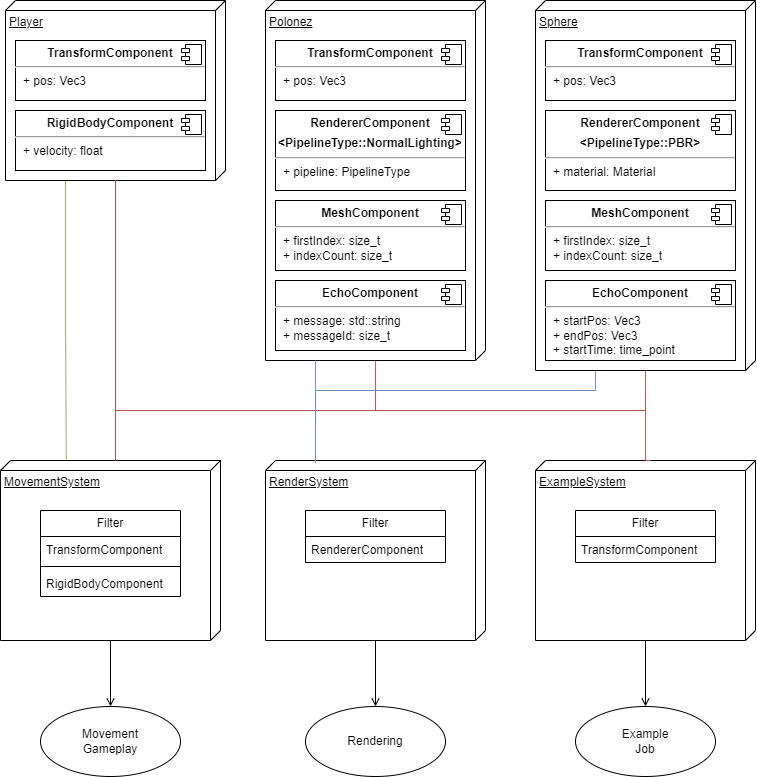
\includegraphics[width=\linewidth]{ecs.png}
  \caption{ECS in work}
\end{figure}

\newpage
\section{Creation of 3D World Immersion}
\[MVP\]
\[MV[2]P[2]\]

\[
\begin{bmatrix}
Orthographic\\
Projection \\
Matrix
\end{bmatrix} 
*
\begin{bmatrix}
X\\
Y\\
Z\\
1\\
\end{bmatrix} 
\]

\[
\begin{bmatrix}
Perspective\\
Projection \\
Matrix
\end{bmatrix} 
*
\begin{bmatrix}
X\\
Y\\
Z\\
1\\
\end{bmatrix} 
\]

\[
a=\frac{h}{w}
\]

\[
f=\frac{1}{tan(\theta / 2)}
\]

\[
\lambda=\frac{zfar}{zfar - znear)}
-
\frac{zfar * znear}{zfar-znear}
\]

\[
\begin{bmatrix}
x\\
y\\
z\\
\end{bmatrix}
\]
Conversion to screen space
\[
\begin{bmatrix}
afx\\
fy\\
\lambda z-\lambda znear\\
\end{bmatrix}
\]
Perspective divide
\[
x/z\ y/z\ z/z
\]

\[
\begin{bmatrix}
(\frac{h}{w})(\frac{1}{tan(\theta/2)}) & 0 & 0 & 0\\
0 & (\frac{1}{tan(\theta/2)}) & 0 & 0\\
0 & 0 & \frac{zfar}{zfar - znear)} & -\frac{zfar * znear}{zfar-znear}\\
0 & 0 & 1 & 0
\end{bmatrix} 
*
\begin{bmatrix}
X\\
Y\\
Z\\
1\\
\end{bmatrix} 
\]

An example of view matrix with camera placed at: 10 5 10:
\[
\begin{bmatrix}
1 & 0 & 0 & -10\\
0 & 1 & 0 & -5\\
0 & 0 & 1 & -10\\
0 & 0 & 0 & 1\\
\end{bmatrix} 
\]

\newpage
\section{Software Testing}
\label{sec:testing}
\hspace{\parindent}
Software development can be a lengthy and convoluted process, so to assure the quality of the project and to prevent hidden errors from disturbing workflow, it is necessary to test the code. There are various methodologies used in the process of software testing, and it is of great importance to be aware of them and best situations to use each of them.
\subsection{Unit Tests}
\hspace{\parindent}
One of the simplest ways for programmers to test their code in development is to use unit tests. This method of software testing focuses on validating the functionality of a single unit or component of the tested code. Usually, unit test are written by the same person or team that coded the feature right after finishing said feature. The main advantage of using unit tests is the ease of implementation and high ratio of finding bugs that are quite obvious but potentially very dangerous for future production. As this type of testing was used in the development of TSEngine, the exact way it was used is described in \hyperref[sec:tests]{\ref*{sec:tests} Tests} section.

\subsection{Smoke Tests}
\hspace{\parindent}
Smoke testing, also known as sanity testing or build verification testing, is a methodology that focuses on quickly checking whether the software has any obvious errors or whether the most basic functionalities work properly. This type of testing is the most suited to determine if the software is ready for more in depth tests, or if it is ready for development of the new features. Although this way of testing was used in the development of TSEngine, there is not any documentation of the process, as it was always a simple check after implementing a new feature.

\newpage
\section{Teamwork}
\label{sec:teamwork}
\hspace{\parindent} % TODO: place here any image to make it more funny like that devops from we used for presentation

As in all projects that involve multiple people, it is crucial to develop a way to share each person's work and to have access to previous iterations of the software. Nowadays, it is of great ease with the emergence of version control systems such as Git or Perforce. 

The TSEngine uses Git and furthermore GitHub to accommodate this problem, as described in detail in \hyperref[sec:scv]{\ref*{sec:scv} Source Control Version} section. Git is released under the open source license -  GNU General Public License version 2.0, and as an open source software is widely used in many sites and platforms: GitHub, GitLab or Bitbucket to name the most popular ones, but there are many more developed and used to accommodate specific needs and preferences of the developers.

Another popular method of version control, although not used in the development of TSEngine, is Perforce, now rebranded as Helix Core. It is a powerful tool used mainly in larger projects by AAA game developers, visual effects studios and semiconductor companies. When using Perforce, one must note that it is proprietary software of Perforce Software, Inc. and is free to use only in teams up to 5 users and 20 workspaces. Perforce is more focused on changing files and is better suited than git when dealing with binary files. As always, in software development it is important to choose the correct tool for the project, and it can make the process of development much easier.

The labor of work we put into the project is explained in \hyperref[]{\ref*{sec:labor} Division Of The Labor}.



